\documentclass{beamer}
\usepackage{graphicx}
\usepackage{hyperref}
\usepackage[sorting=none]{biblatex}
\bibliography{refs}
\usepackage{tikz}
\usetheme{Madrid}
\definecolor{ginger}{rgb}{0.69, 0.4, 0.0}
\usecolortheme{beaver}
\titlegraphic{
\includegraphics[width=2.5cm]{logo.png}
}
\title[Interaction of Laser Pulse With Plasma]{Interaction of Laser Pulse With Plasma}
\date{}
\institute[IIT Delhi]{\large Indian Institute of Technology, Delhi}
\author[]{Kulwinder Kaur (2021PHS7190)\\ Harikesh Kushwaha (2021PHS7181)\\[3mm]Adviser: Prof. Vikrant Saxena}
\vspace{0cm}
\begin{document}
\maketitle
\begin{frame}{Introduction}
    \frametitle{Introduction}
    \small
    Interaction of light with matter at Ultra High Light intensity gives access to novel physical regimes which are barely, if at all, explored in lab.\cite{henri}
    \begin{itemize}
        \item Intensity of laser in order of $10^{23} \; W/cm^{-2}$ has been reached experimentally.\cite{highintensity}.
        \item QED effects starts acting at intensity above $10^{25}W/cm^{-2}$.
        \item Intensity level of $10^{29}W/cm^{-2}$ corresponds to the Schwinger field.
    \end{itemize}
    % Intensity of laser in order of $10^{23} \; W/cm^{-2}$ has been reached experimentally with the CoReLS petawatt (PW) laser.\cite{highintensity}. The next step is to push forward these intensities above $10^{25}W/cm^{-2}$. Above this limit, quantum electrodynamics effects start playing a major role on the dynamics of electrons. Intensity level of $10^{29}W/cm^{-2}$ corresponds to the Schwinger field. At this field, light starts generating electron positron pair out of vacuum. Vacuum starts acting like a nonlinear medium and its refractive index becomes a function of light intensity. These physical regimes are barely, if at all, explored in lab.
    Here, we study the generation of high harmonics of the incident laser pulse by its interaction with overdense plasma.

    \begin{itemize}
        \item Plasma is overdense if its density is so high that it reflects the incident laser pulse.
        \item The em field of the incident laser pulse drives relativistic oscillations in the plasma electrons which results in the generation of high harmonics.
        \item Simulations are performed to study the effect of some plasma and laser parameters on high harmonics generation.
        \item Oscillations of the plasma surface is also studied.
    \end{itemize}

    % Here, the generation of harmonics of incident laser pulse by interaction of a high intensity laser pulse with a step boundary overdense plasma layer is studied and the effect of variuos parameters on the generated high hormonics is investigated. For this, fully relativistic particle in cell simulations are performed using \textit{EPOCH}. Already, variuos experiments and simulations have been performed to study how high hormonics are changed by using different polarization of laser pulse \cite{polarization1} \cite{polarization2}, different PM shapes \cite{henri}, two color laser pulses \cite{two-color1} \cite{two-color2}. In this article, we study the effect of plasma density, laser intensity, envelope and pulse duration on generated high harmonics.

\end{frame}

\begin{frame}
    \frametitle{Simulation Parameters}
    \small
    The simulation uses \textit{EPOCH}, a parallised, second order and fully relativistic implementation of particle in cell algorithm.\cite{EPOCH} The current simulation is performed in 1D3V only. We want to study the effect of various plasma and laser parameters on the generated high harmonics. The parameters which are constant throughout the entire experimentation are these:
    \begin{itemize}
        \item The simulation box extends for $40 \lambda _l$ (from $-20 \lambda _l$ to $20 \lambda _l$), $\lambda_l = 1 \mu m$
        \item Number of cells is 16000 and the plasma is placed at $x=0$ and with a thickess of $\lambda_l$. There are 100 particles per cell.
        \item Pulse duration is  $T = 20 \tau$ and simulation is run till $T_{end} = 40 \tau$. $\tau$ is time period of laser pulse $\approx 3.3 fs$
    \end{itemize}
    % The simulation box extends for $40 \lambda _l$ (from $-20 \lambda _l$ to $20 \lambda _l$), where $\lambda_l$ is the laser wavelength taken as $1\mu m$ and has total 16000 cells, i.e., 400 cells per wavelength. The plasma is placed at $x=0$ and with a thickess of $\lambda_l$. Number of particles per cell are 100.
    % For most of the simulations the pulse duration is $T = 20 \tau$ and simulation is run till $T_{end} = 40 \tau$. Here $\tau$ is the time period of laser pulse.\\
    Some parameters are varied to study their effect on the generated high harmonics. These parameters and their effect on the harmonics are discussed in the next section.

\end{frame}

\begin{frame}
    \frametitle{Effect of Plasma Density and Laser Intensity}
    % \begin{minipage}[t]{0.48\linewidth}
    %     left part
    % \end{minipage}
    % \begin{minipage}[t]{0.48\linewidth}
    %     right part
    % \end{minipage}
    \begin{figure}
        \centering
        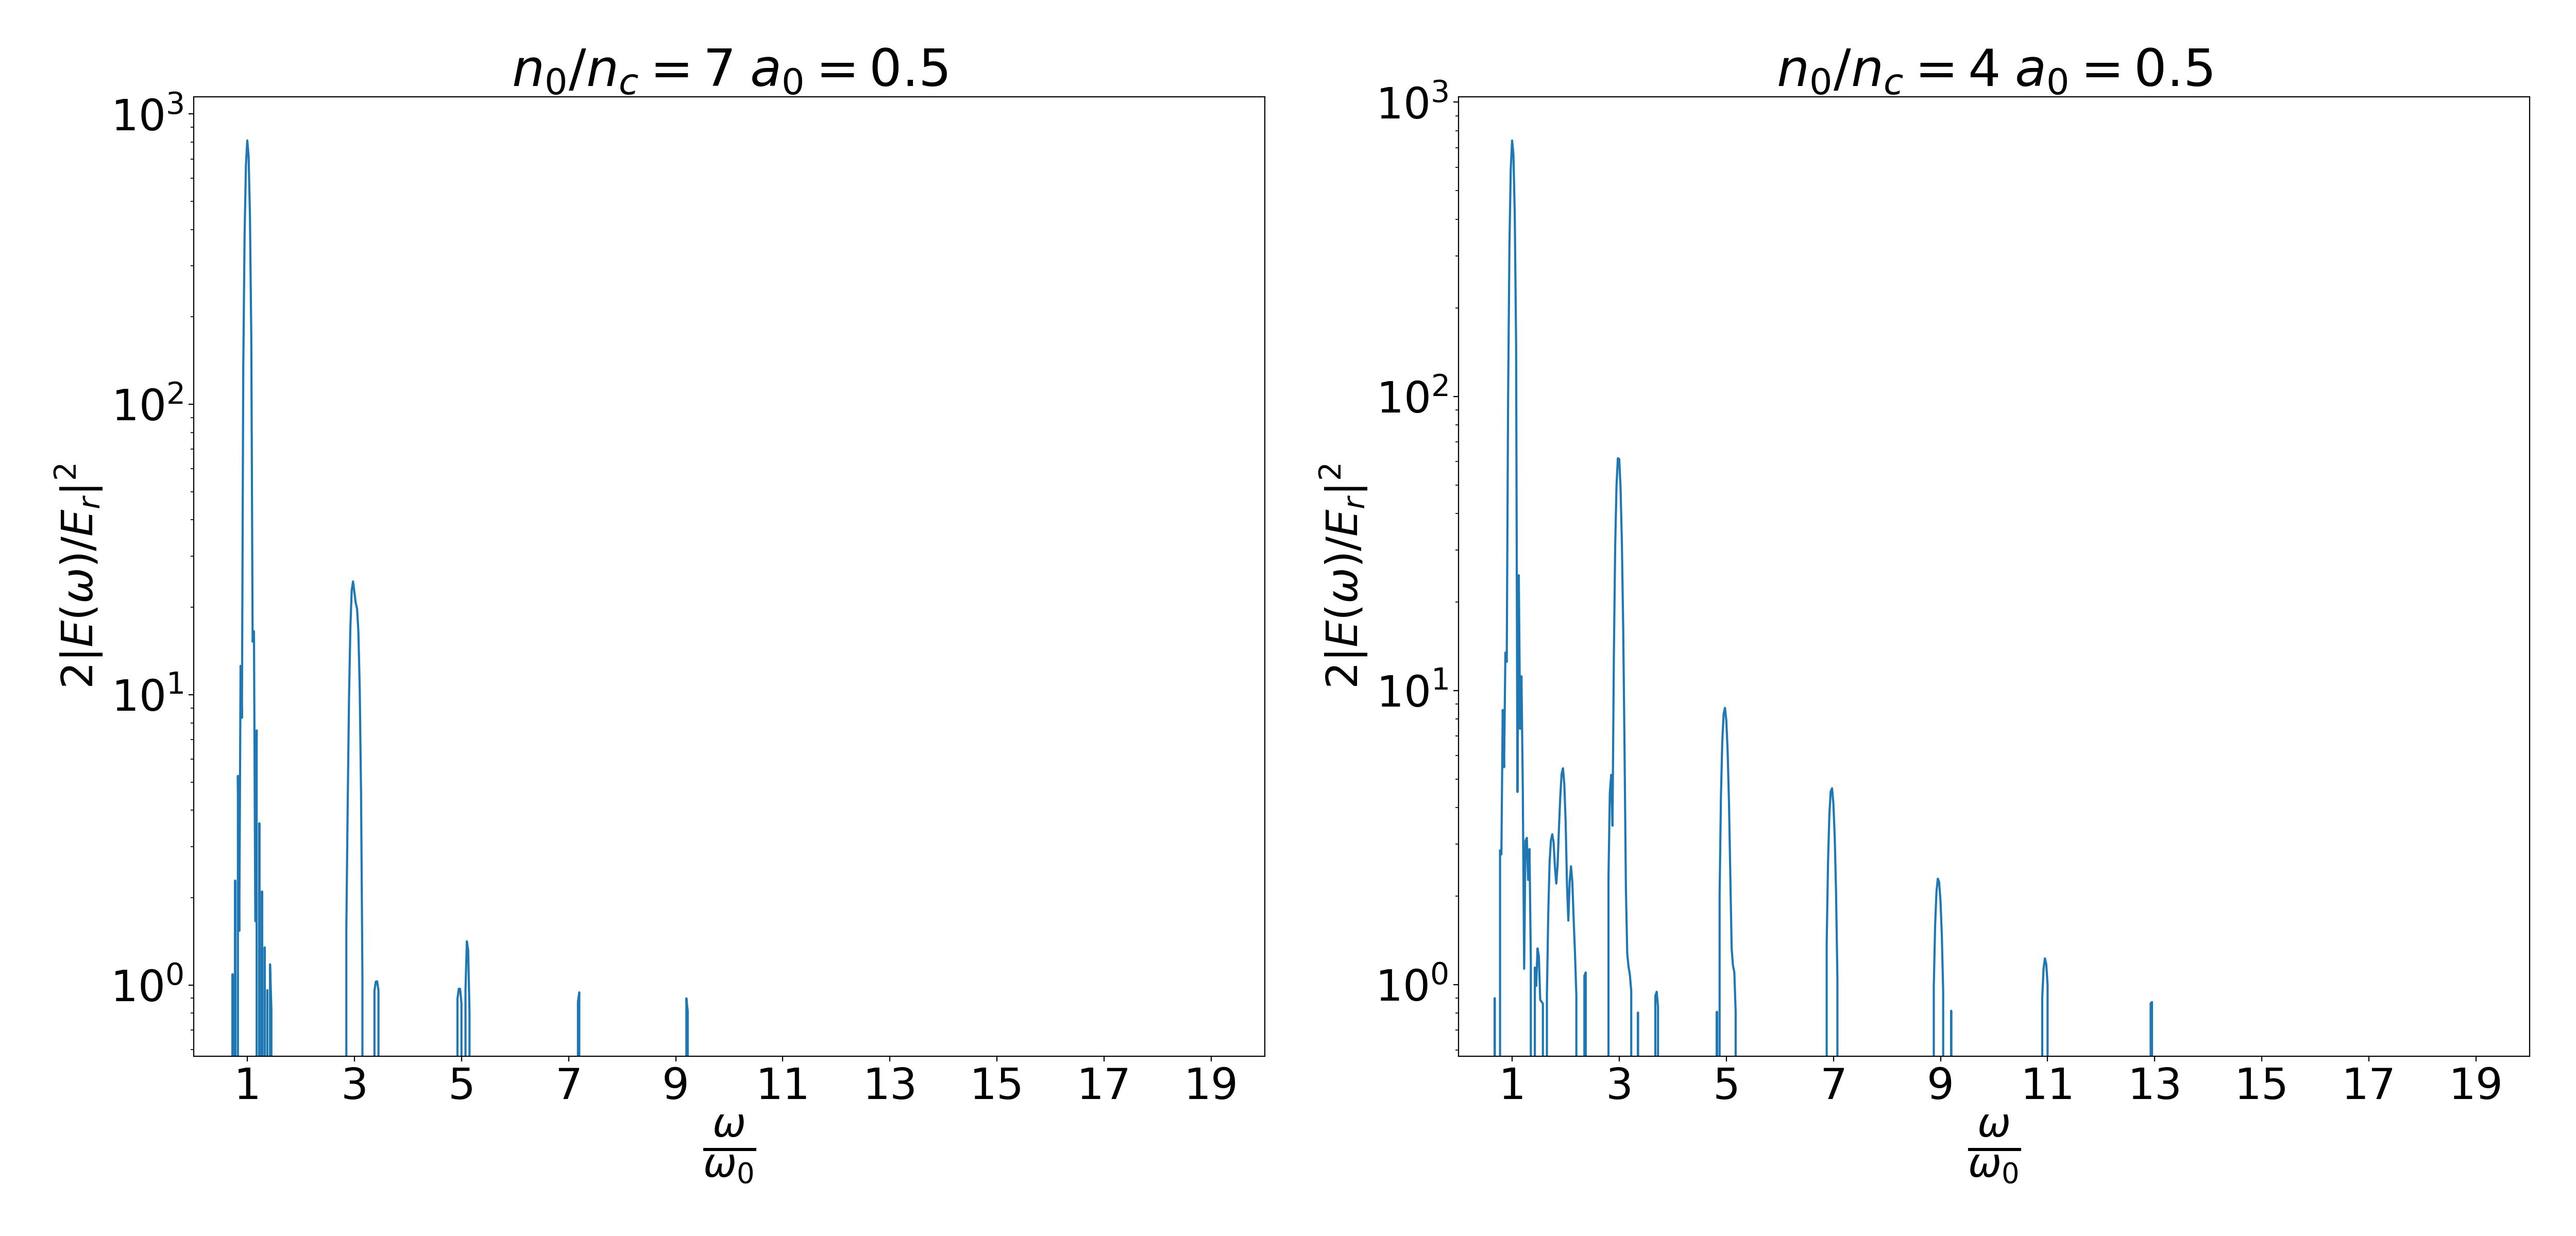
\includegraphics[width=1.0\textwidth, height=0.4\textheight]{images/density.jpg}
        % \caption{Effect of plasma density on generated harmonics}
        \label{fig:PlasmaDensity}
    \end{figure}
    \begin{figure}
        \centering
        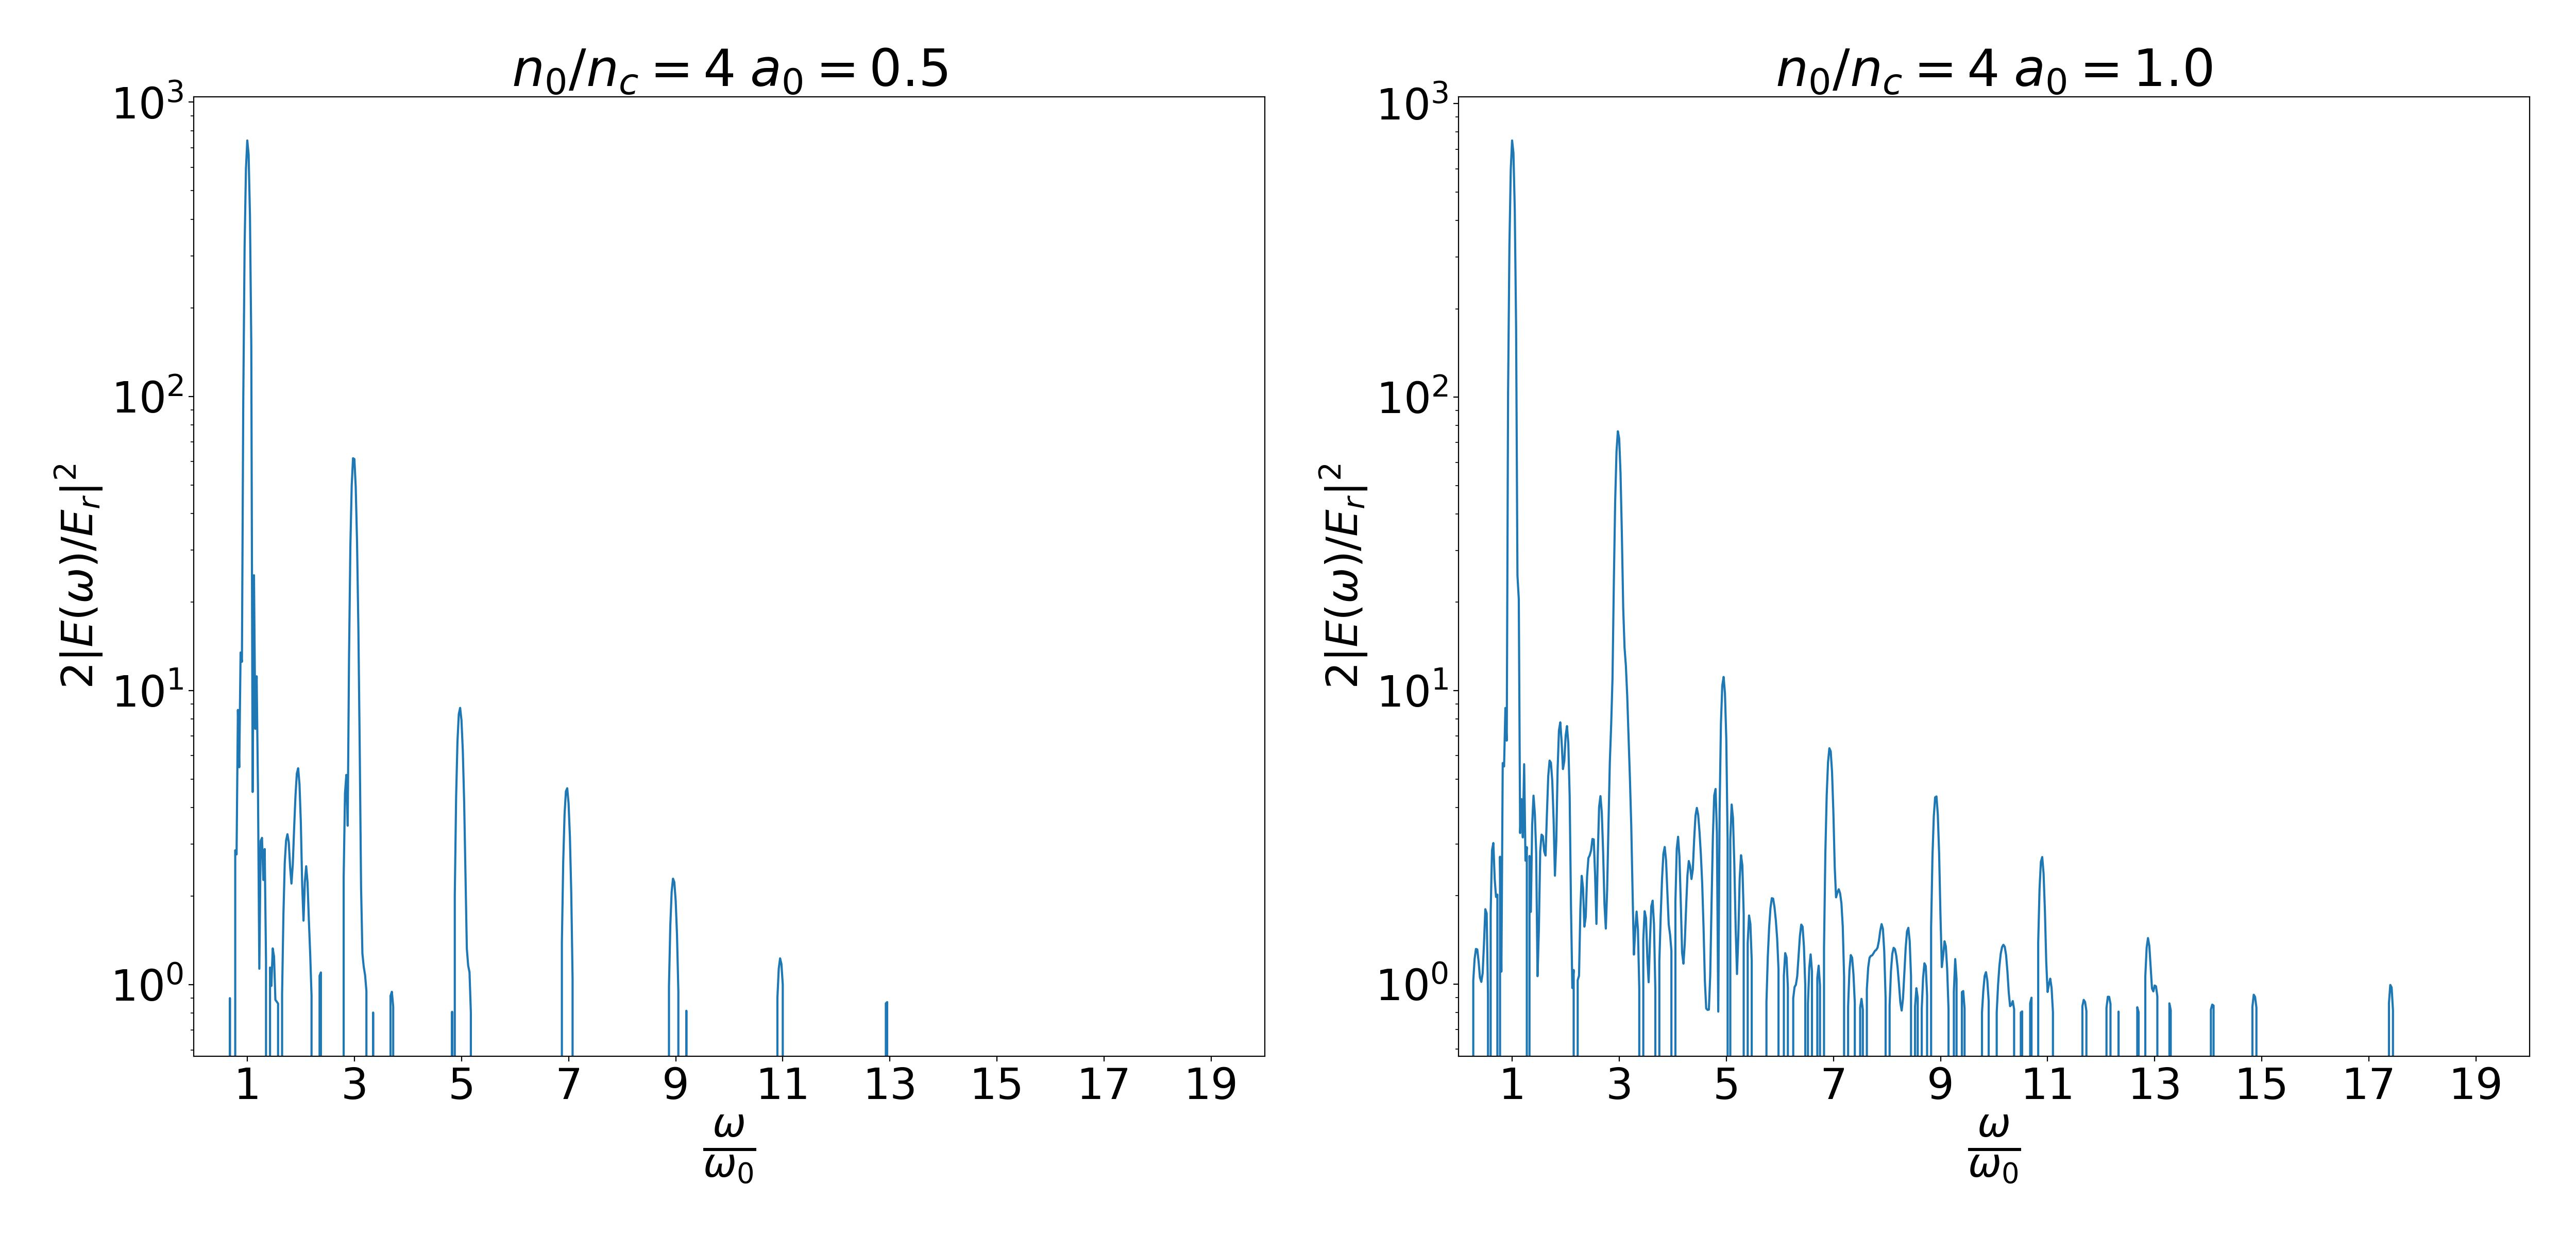
\includegraphics[width=1.0\textwidth, height=0.4\textheight]{images/intensity.jpg}
        % \caption{Effect of plasma density on generated harmonics}
        \label{fig:LaserIntensity}
    \end{figure}
\end{frame}

\begin{frame}
    \frametitle{Effect of Laser Envelope}
    \tiny
    \begin{minipage}[t]{0.35\linewidth}
        1. Sine Sqaured
        \begin{equation*}\label{sin-sq-env}
            P(t)=
            \begin{cases}
                 & \sin^2(\pi t/T) \text{ for } 0 \leq t \le T \\
                 & 0         \;      \text{ otherwise }
            \end{cases}
        \end{equation*}
        2. Gaussian
        \begin{equation*}\label{gaussian-env}
            P(t)=
            \begin{cases}
                 & e^{\frac{-(t-T/2)^2}{2(0.2T)^2}} \text{ for } 0 \leq t \le T \\
                 & 0         \;      \text{ otherwise }
            \end{cases}
        \end{equation*}
        3. Triangular
        \begin{equation*}\label{triangle-env}
            P(t)= 2\times
            \begin{cases}
                 & t/T \text{ for } 0 \leq t \le T/2    \\
                 & 1-t/T \text{ for } T/2 \leq t \le T  \\
                 & 0         \;      \text{ otherwise }
            \end{cases}
        \end{equation*}
    \end{minipage}
    \begin{minipage}[t]{0.64\linewidth}
        \begin{figure}
            \centering
            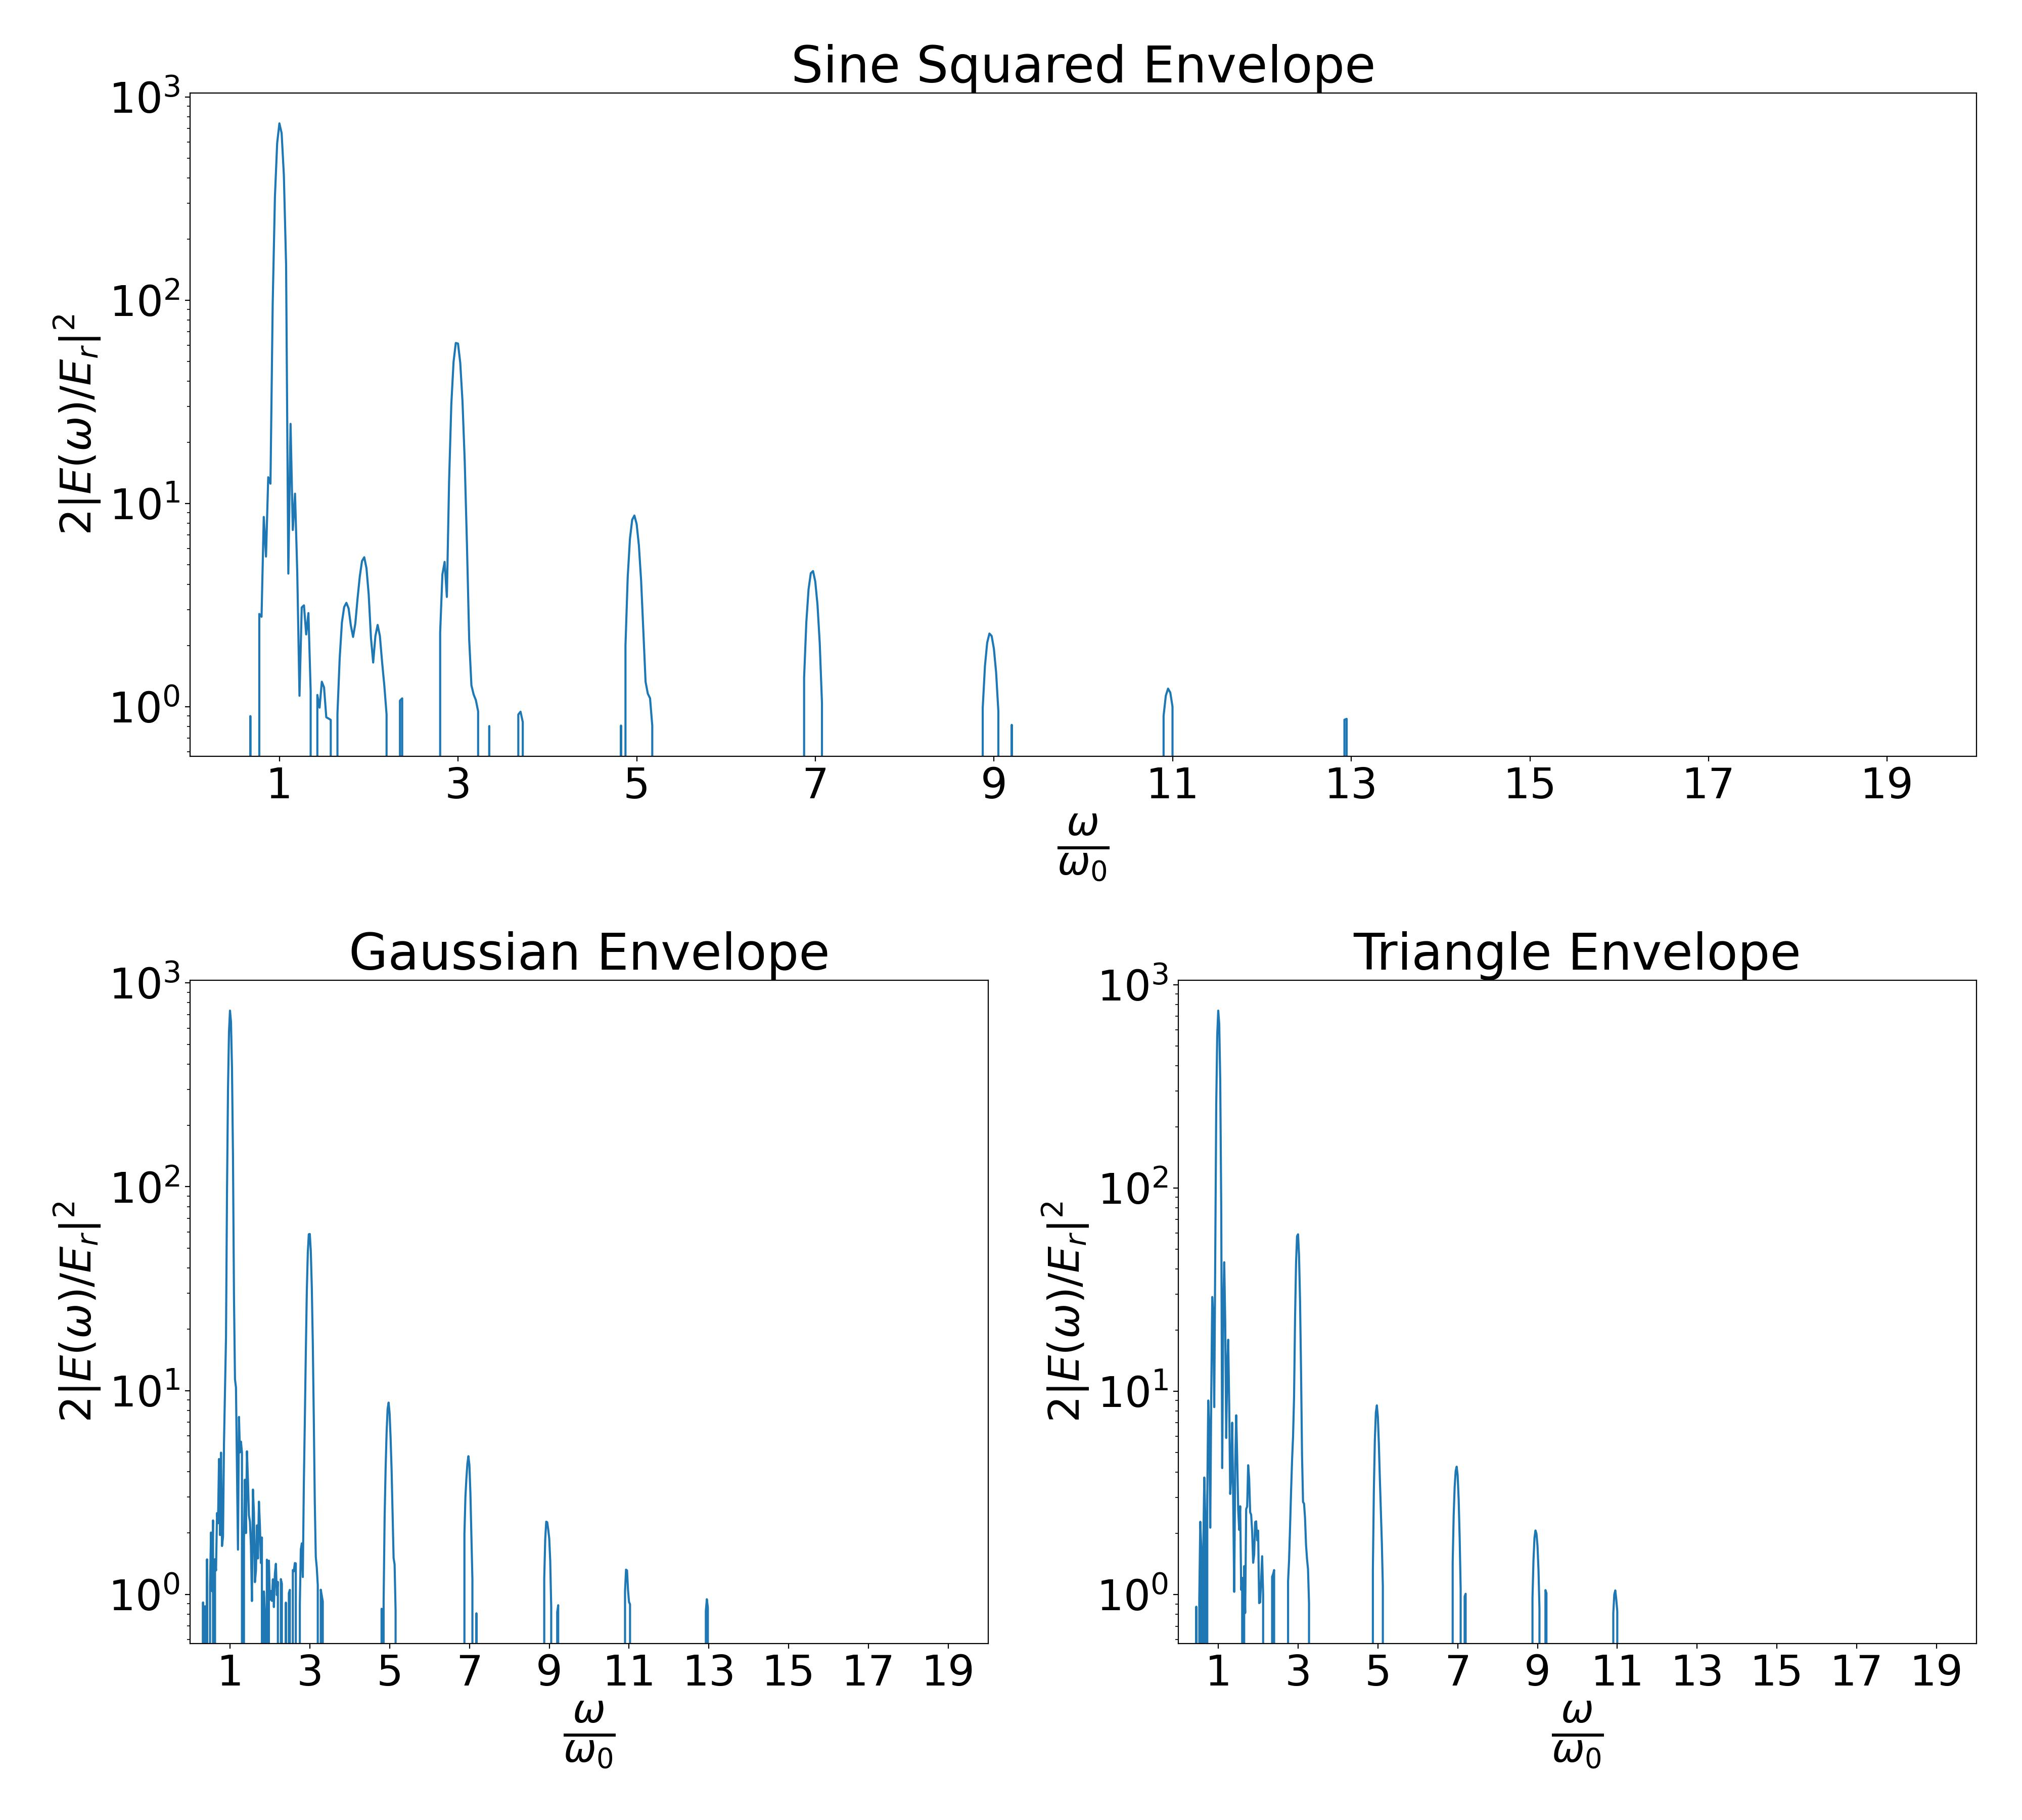
\includegraphics[width=1.0\textwidth, height=0.8\textheight]{images/env.jpg}
            % \caption{Effect of plasma density on generated harmonics}
            \label{fig:LaserEnv}
        \end{figure}
    \end{minipage}

\end{frame}

\begin{frame}
    \frametitle{Effect of Pulse Length}
    \begin{figure}
        \centering
        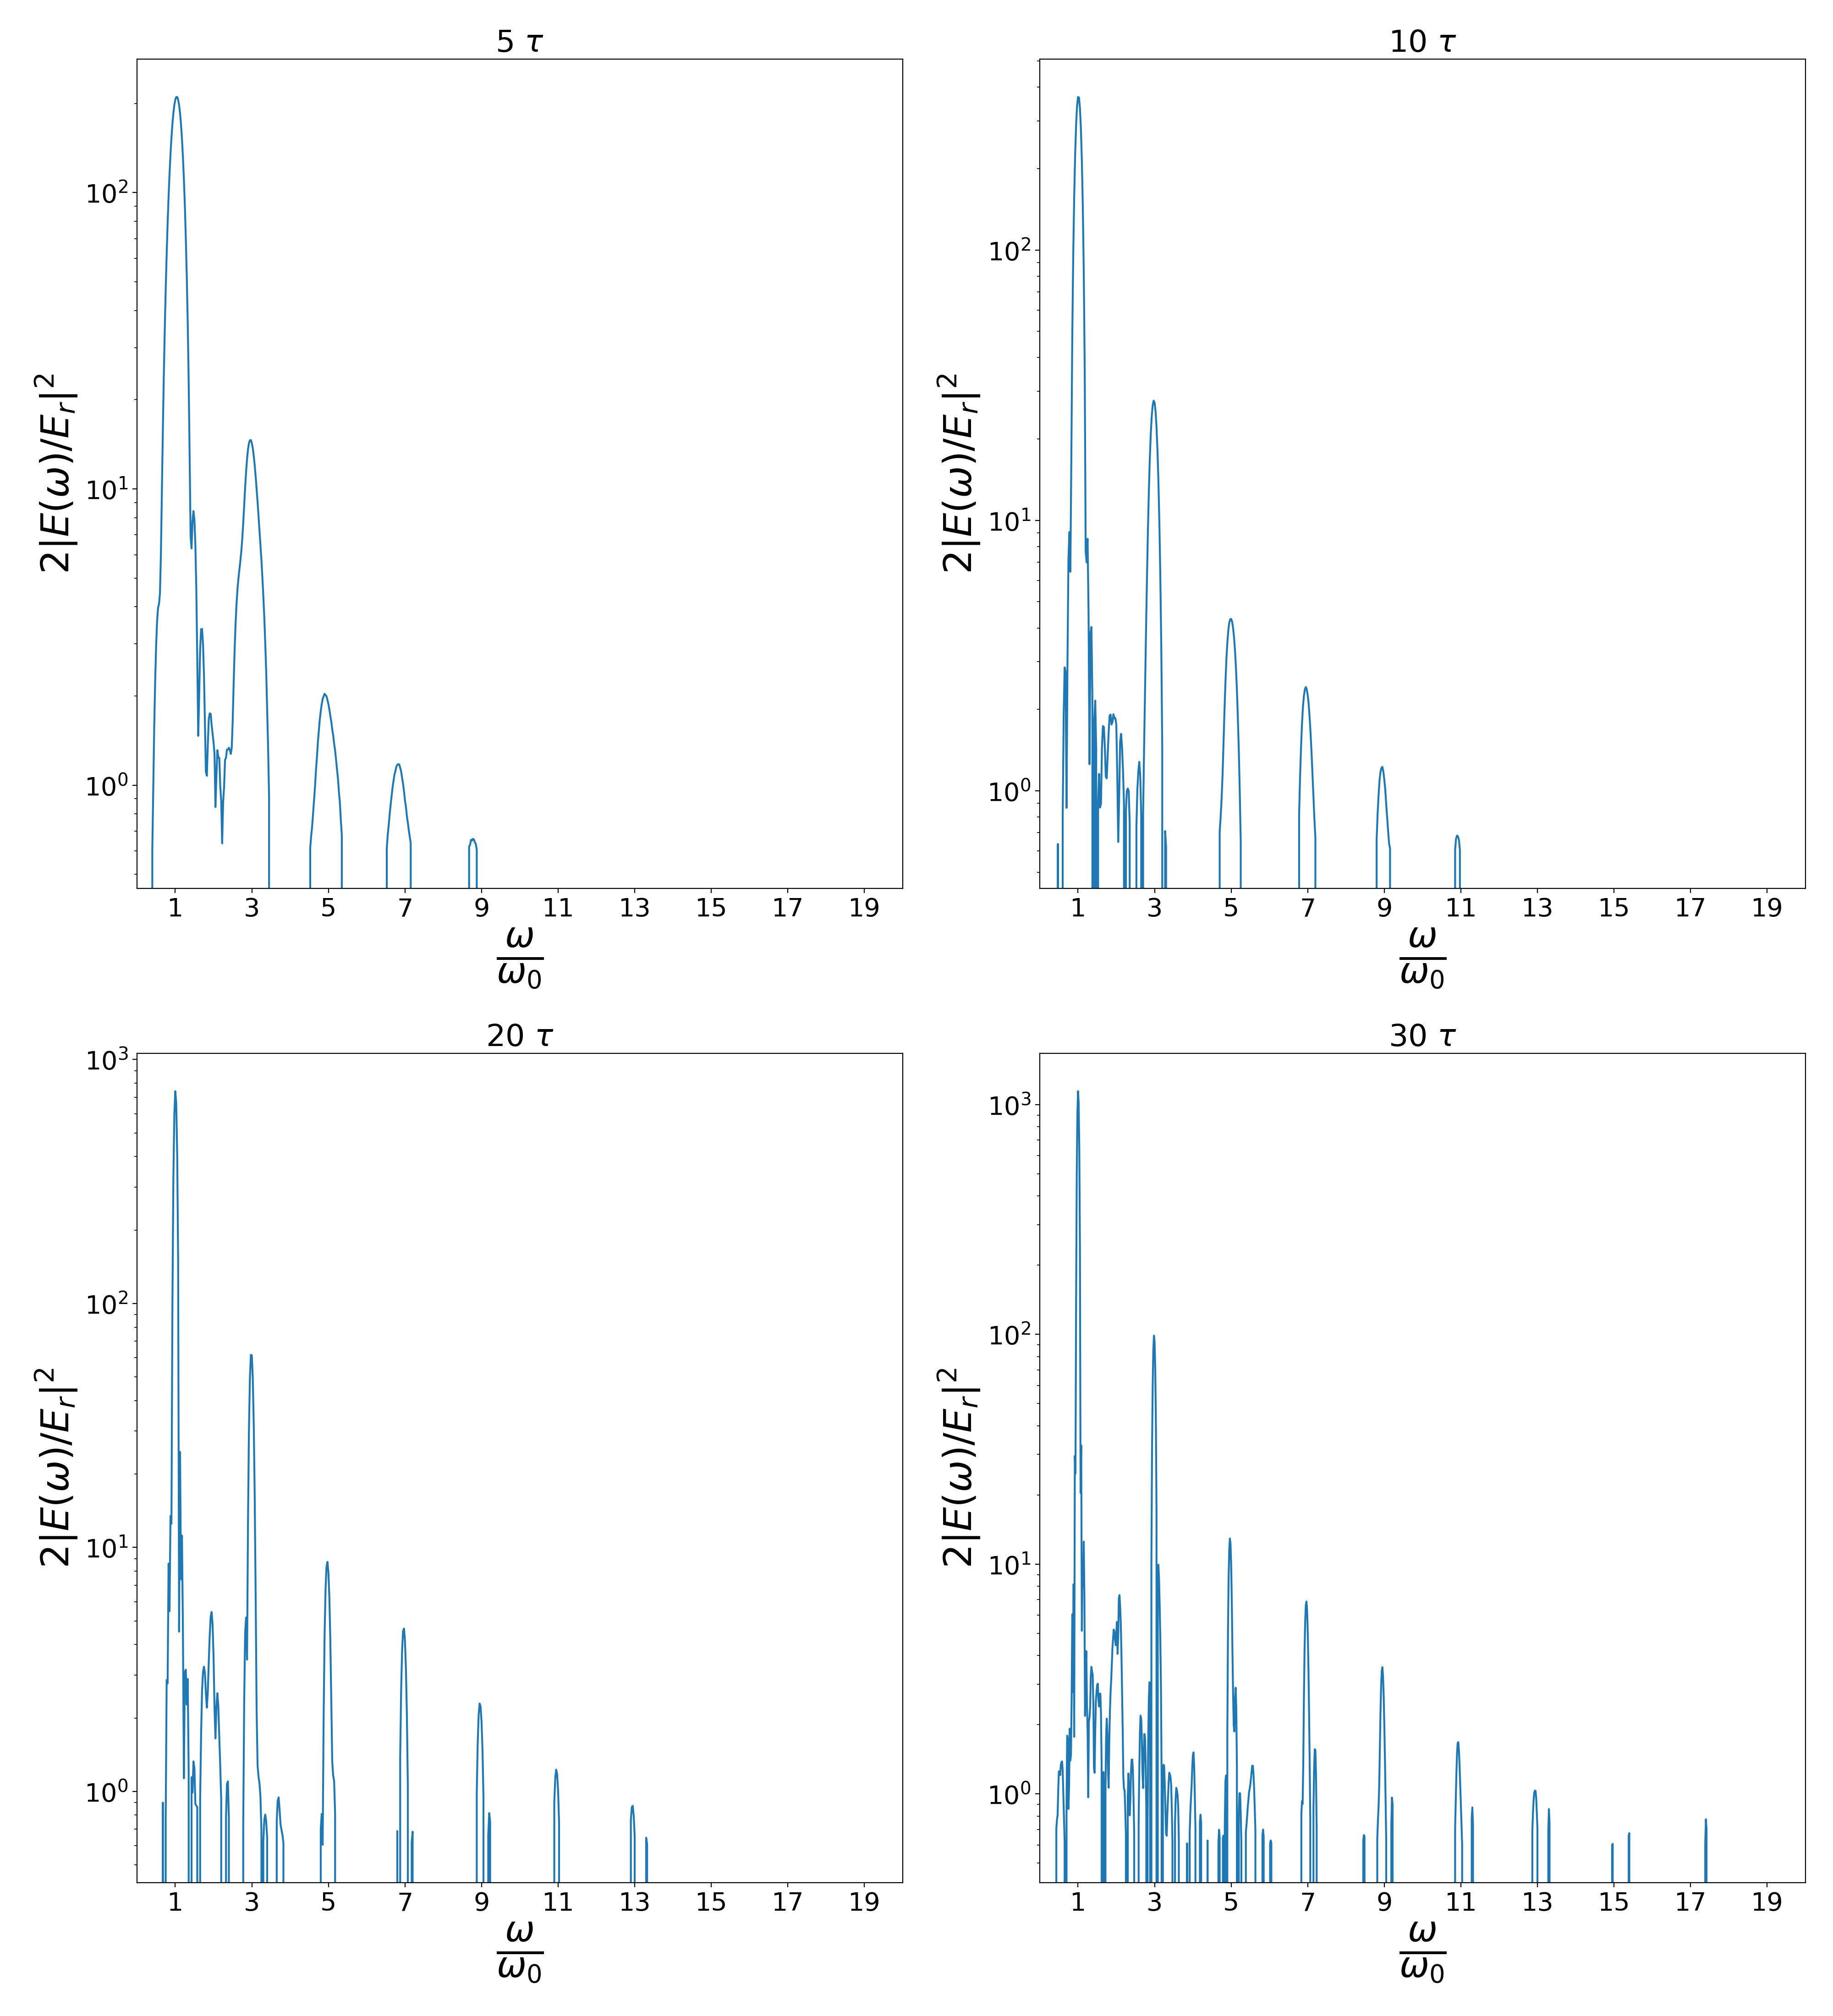
\includegraphics[width=1.0\textwidth, height=0.8\textheight]{images/pulse.jpg}
        % \caption{Effect of plasma density on generated harmonics}
        \label{fig:LaserPulsev}
    \end{figure}
\end{frame}
\begin{frame}
    \frametitle{Effect of Laser Intensity on Electron Oscillations}
    \begin{figure}
        \centering
        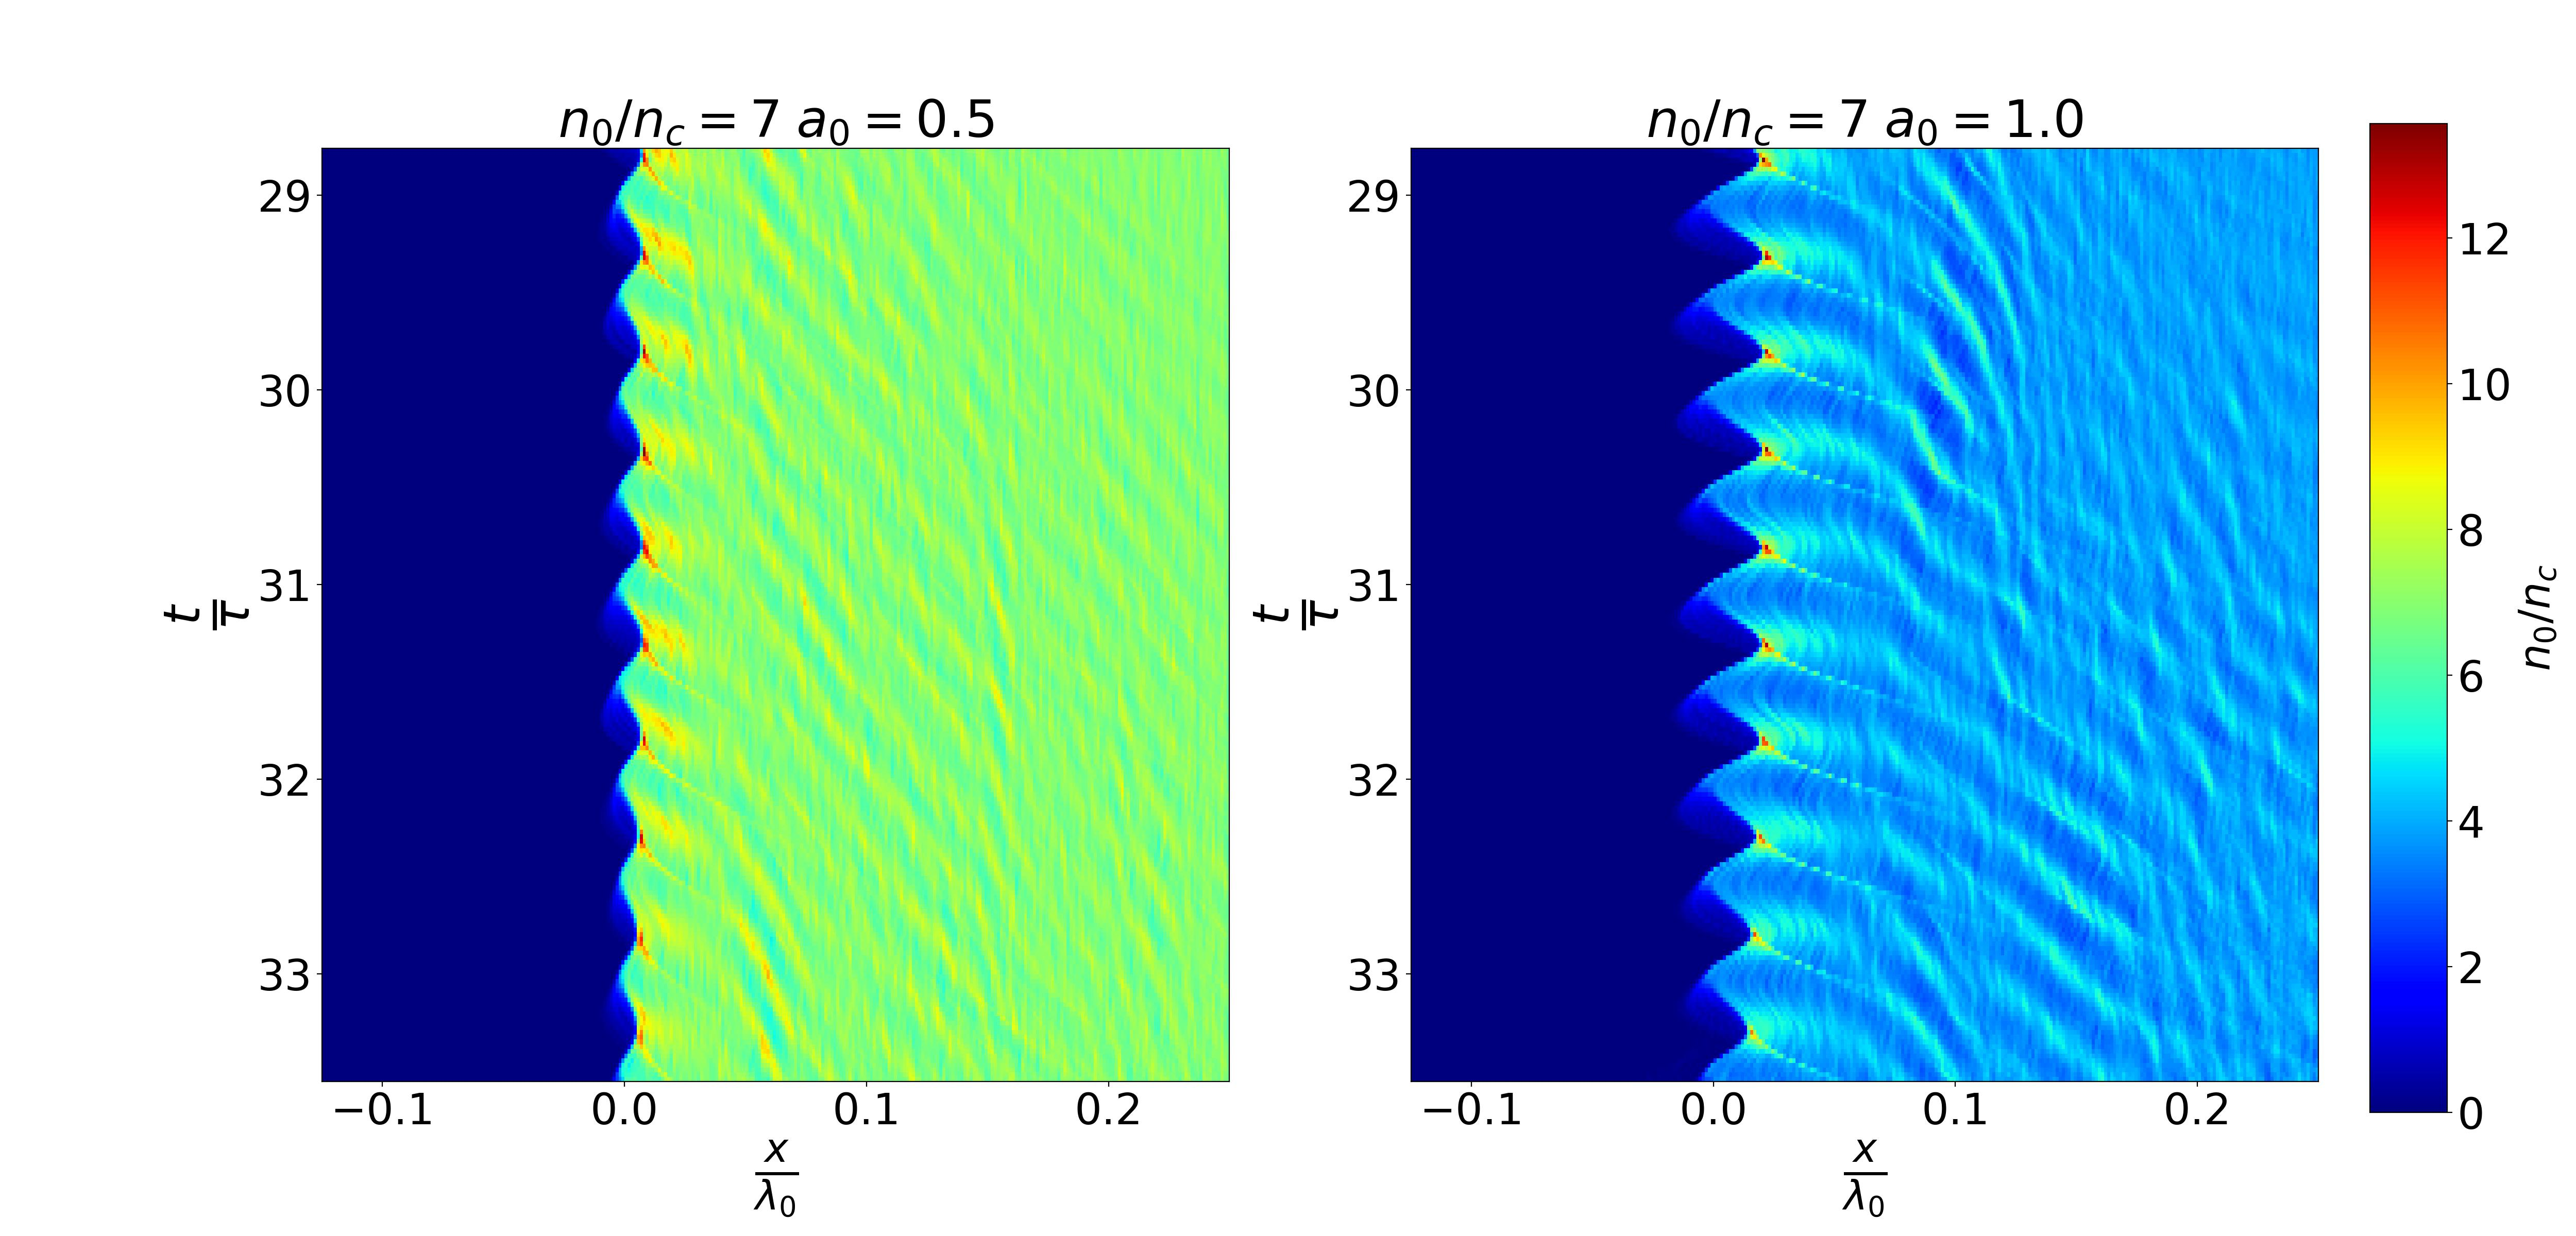
\includegraphics[width=1.0\textwidth, height=0.8\textheight]{images/oscillation1.jpg}
        % \caption{Effect of plasma density on generated harmonics}
        \label{fig:Oscillations1}
    \end{figure}
\end{frame}

\begin{frame}
    \frametitle{Frequency of Oscillations}
    \begin{figure}
        \centering
        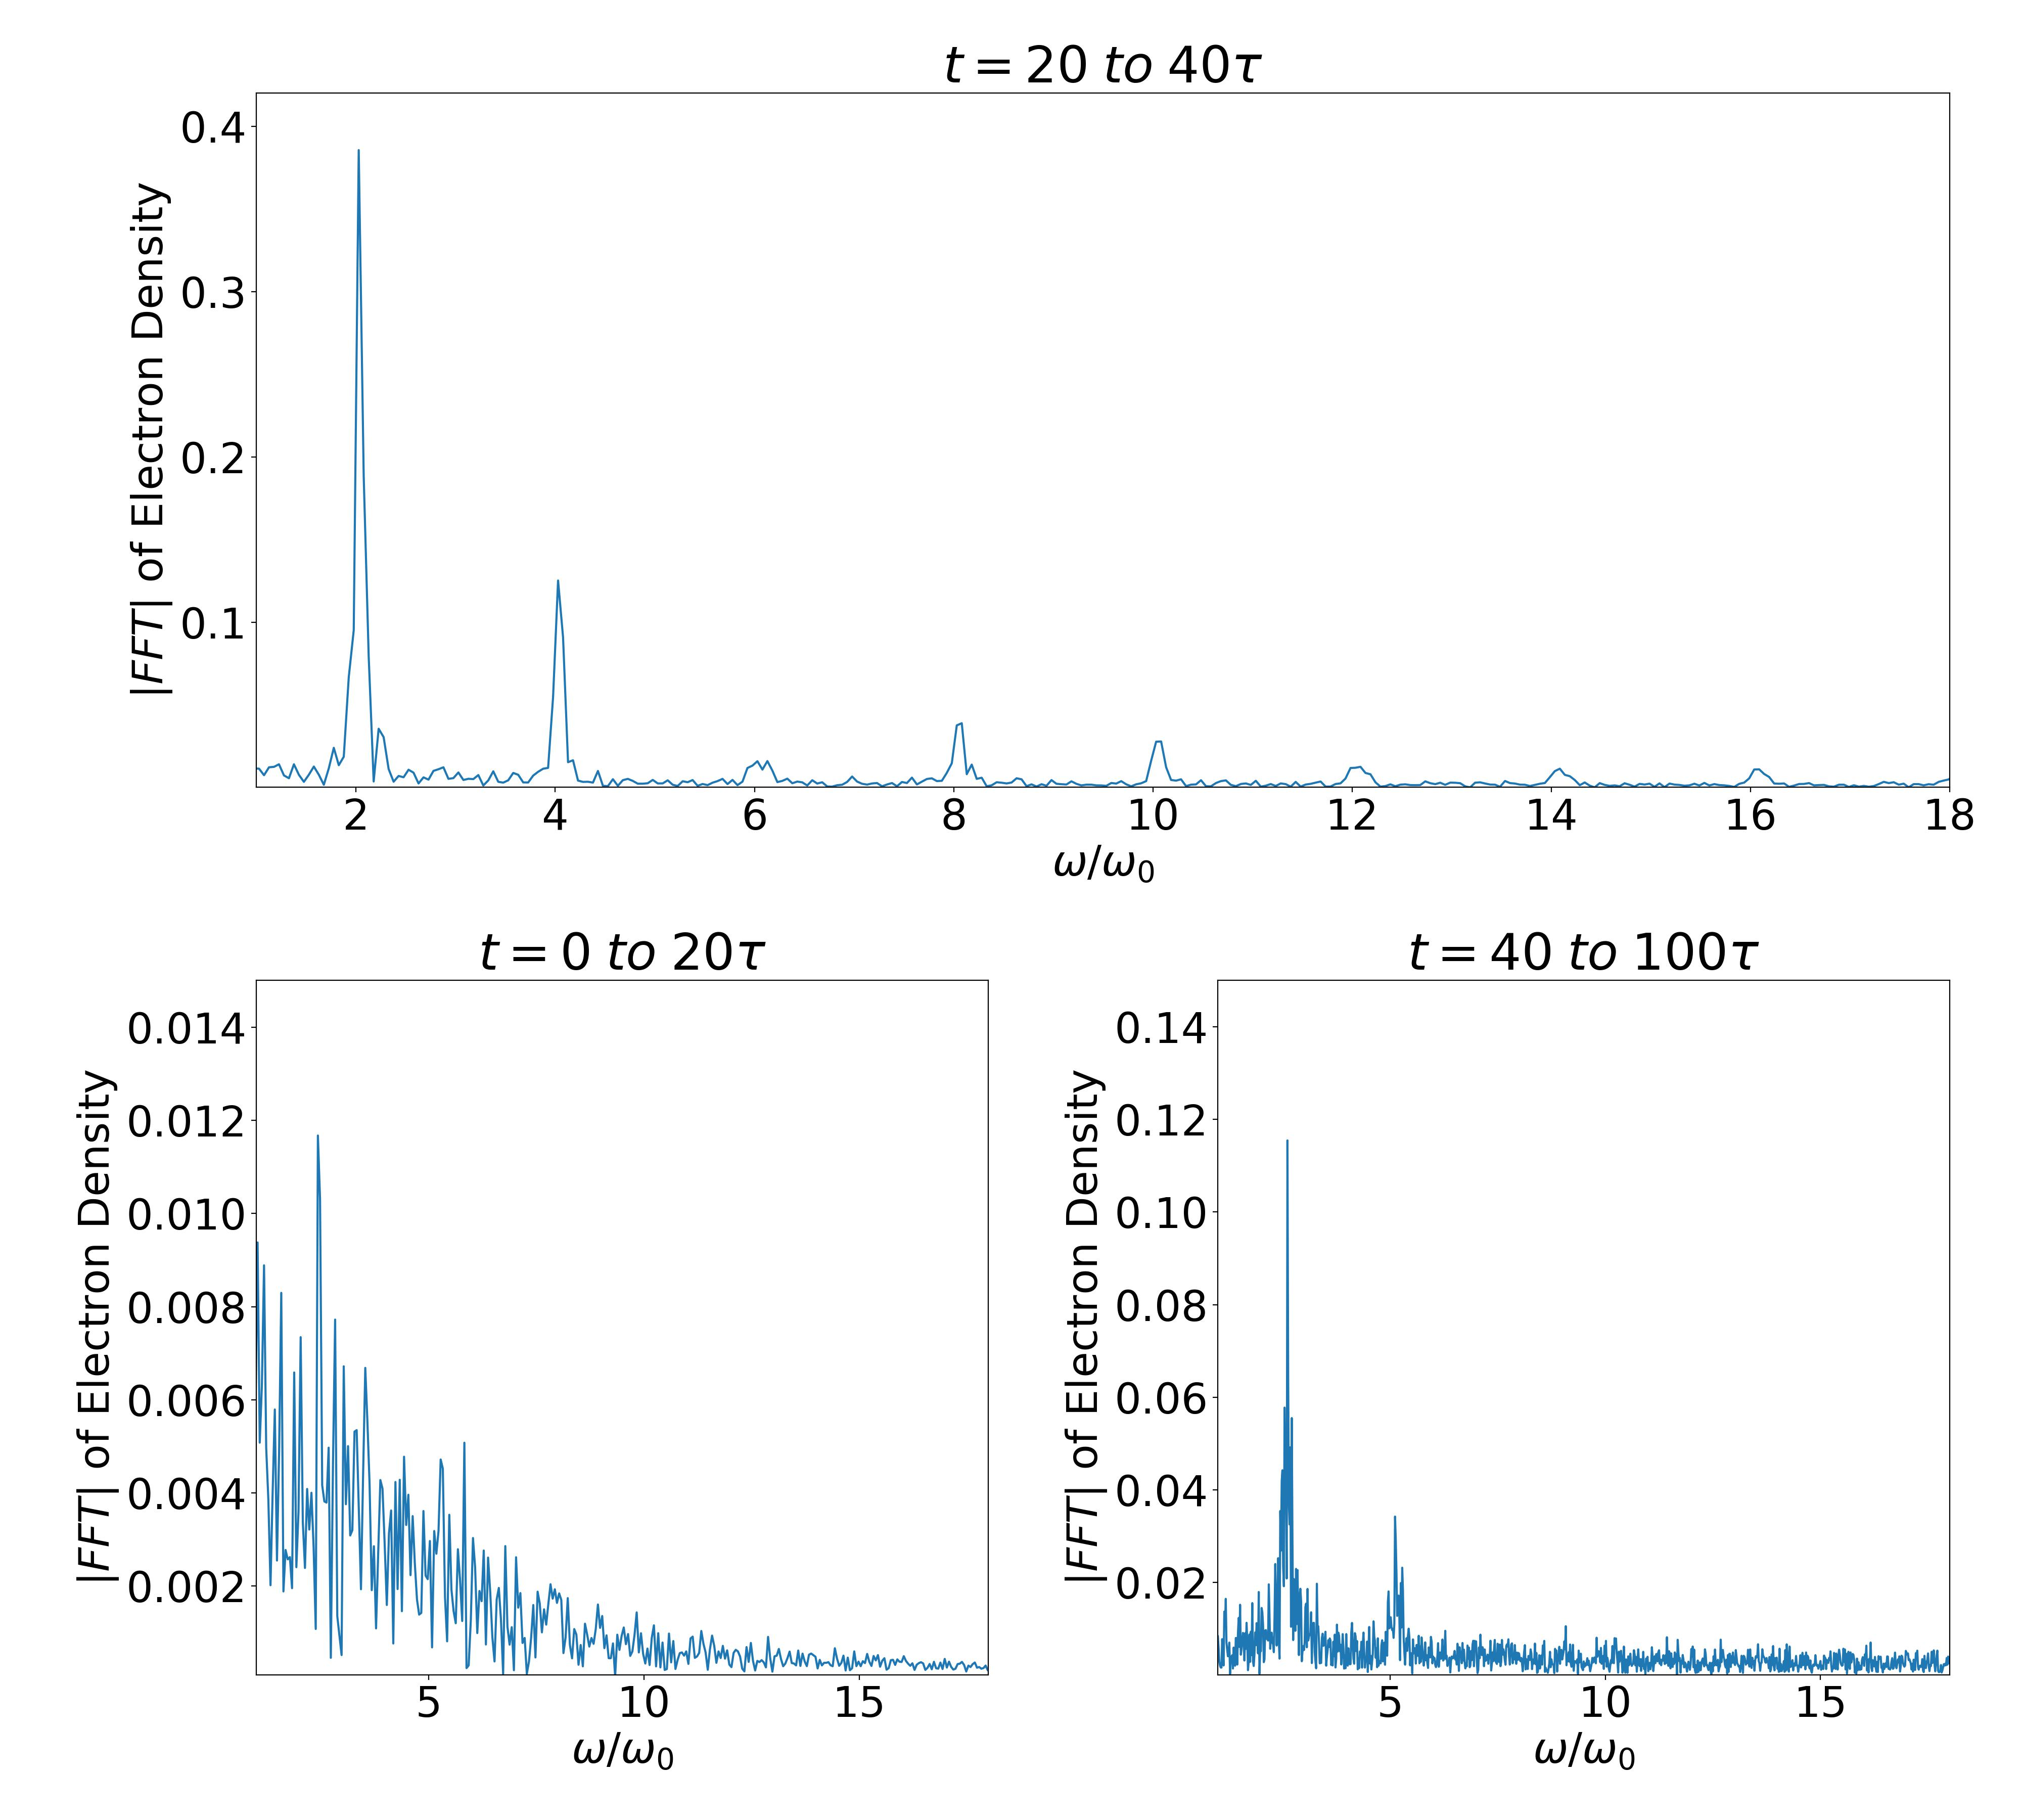
\includegraphics[width=0.8\textwidth, height=0.8\textheight]{images/oscillation2.jpg}
        % \caption{Effect of plasma density on generated harmonics}
        \label{fig:Oscillations2}
    \end{figure}
\end{frame}
\begin{frame}
    \frametitle{Current Status and Future Plan of Work}
    The interaction of high intensity laser pulse with overdense plasma is investigated. During this, odd harmonics of the incident laser pulse is generated and the effect of variuos laser and plasma parameters on the hormonic generation is studied. Future plan of work is to study about the effects of some more parameters on the harmonics generation escpecially the effect of oblique incidence and different polarization of the laser pulse.
\end{frame}

\begin{frame}
    \AtNextBibliography{\small}
    \printbibliography
\end{frame}
\end{document}